\section{DFDs}
A data flow diagram (DFD) is a graphical representation of the "flow" of data through an information system, modeling its process aspects. A DFD is often used as a preliminary step to create an overview of the system, which can later be elaborated. DFDs of DoS is as following-:

\begin{figure}[ht]
\centering
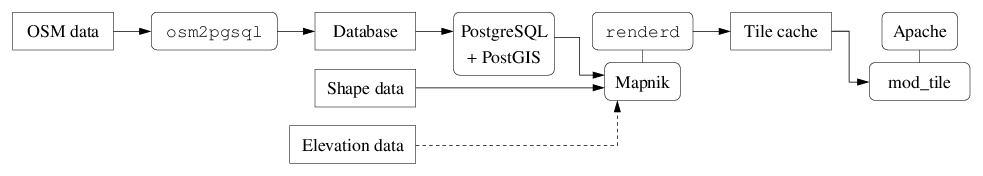
\includegraphics[scale=0.6]{input/images/osmserv.png}
\caption{Data Flow Of Whole System}
\end{figure}
\section{Flowchart}
A flowchart is a type of diagram that represents an algorithm, work flow or process, showing the steps as boxes of various kinds, and their order by connecting them with arrows
and following are flowchart of DoS showing flow of control and Data in the software-:
\begin{figure}[ht]
\centering
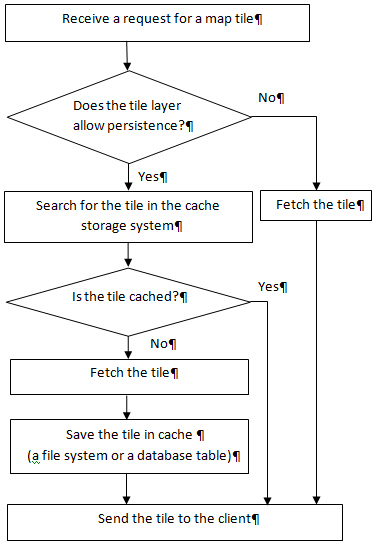
\includegraphics[scale=0.9]{input/images/fetch.jpg}
\caption{Flow Chart to Serve a Tile}
\end{figure}
\hspace{-1.7em}



\section{Problem Formulation}
Geographical data (geo data) is not free in many parts of the world.\\
Because that data is copyrighted and owned by multiple organisations like the Ordnance Survey. Google/whoever just licenses it. If we were to use it, we'd have to pay for it. \\
\noindent "OpenStreetMap is a free editable map of the whole world. It is made by people like you." Which means the database will always be subject to the whims, experimentation, and mistakes of the community. This is precisely OSM's strength since, among other things, it allows our data to quickly accommodate changes in the physical world.\\
\noindent By making your system an OSM tile server not only you can edit the map but can use it offline also. You can change the styling of the map like color of the roads fonts style and amny more as per your requirments. 

%\section{Types of Feasibility Study}
%\noindent Feasibility analysis involved a thorough assessment of the operational and technical aspects of the proposal.
%Feasibility study tested the system proposal and identified whether the user needs may be satisfied using
%the current software and hardware technologies, whether the system will be cost effective from a business
%point of view and whether it can be developed with the most up to date technologies.
%\subsection{Operational Feasibility}
%\noindent Operational feasibility is a measure of how well a project solves the problems, and takes advantage of
%the opportunities identified during scope definition and how it satisfies the requirements identified in
%the requirements analysis phase of system development. All the operations performed in the software
%are very quick and satisfy all the requirements.
%\subsection{Technical Feasibility}
%\noindent Technological feasibility is carried out to determine whether the project has the capability, in terms
%of software, hardware, personnel to handle and fulfill the user requirements. The assessment is based
%on an outline design of system requirements in terms of Input, Processes, Output and Procedures.
%OpenStreetMap is technically feasible as it is built up using various open source technologies and it can run on any platform.
%\subsection{Economic Feasibility}
%\noindent Economic analysis is the most frequently used method to determine the cost/benefit factor for evalu-
%ating the effectiveness of a new system. In this analysis we determine whether the benefit is gained
%according to the cost invested to develop the project or not. If benefits outweigh costs, only then
%the decision is made to design and implement the system. It is important to identify cost and benefit
%factors, which can be categorized as follows:
%\begin{itemize}
%\item Development Cost
%\item Operation Cost
%\end{itemize}
%This System is Economically feasible with 0 Development and Operating Charges
%as it is developed in Qt Framework and libdxfrw library which is open source technology and is available free of cost on the internet.

\section{Dependencies}
%\subsection{Hardware Requirements}
\begin{itemize}
\item Operating System: Linux/Windows
\item Processor Speed: 512KHz or more
\item RAM: Minimum 2GB
\item Library: Mapnik
\item Modules: Mod\_tile
\item Compiler: CartoCSS
\item Stylesheet: OSMBright
\item Programming Language: C++, Python
\end{itemize}
%\subsection{Software Requirements}
%\begin{itemize}
%\item Library: Mapnik
%\item Modules: Mod\_tile
%\item Compiler: CartoCSS
%\item Stylesheet: OSMBright 
%\item Programming Language: C++, Python 
%\end{itemize}

\section{Methodology}
\begin{itemize}
\item Studying various methods available to solve different problems of numerical analysis.
\item Deciding various input and output parameters of methods.
\item Making the approach modular 
\item Styling the map.
\item Generating documentation
\end{itemize}

\section{Project Work} 
\textbf{Studied Previous System:}\\
Before starting the project, \\\\
\textbf{Learn Linux:}\\
Before starting with project, we have to install various things to make our system an OSM server. So, for that you should know terminal commands because I gonna explain it for Ubuntu only. It is possible on other OS also but you have to work it own. I have provided some basic command also for Linux. \\\\
\textbf{Learn Postgresql:}\\
 We have to go through the basics of postgresql(database) also, such that there
should not be any problem proceeding with project.\\\\
\textbf{Make or Cmake}\\
The softwares like mapnik, mod\_tile, osm2pqsql, are compiled through the Cmake which is basically language. So, we should the basics of it.
\\\\
\textbf{Languages:}\\
We should the basics of the languages like C++, javascript, python etc for manuplating the stylying and rendering of the map.\\\\
\textbf{Input:}\\
Input values are taken from user or default values defined in the file are used.\\\\
\textbf{Output:}\\
According to input values we will get the particular location of the map.

